% % % % % % % % % % % % % % % % % % % % % % % % % % % % % % % % % % % % 
% 
% FS-Vorlage											Stand: 30.01.12
%
% Formelsammlungsvorlage von Emanuel Regnath und Martin Zellner	
% Bietet verschiedene Abkürzungen und Befehle	
%
% % % % % % % % % % % % % % % % % % % % % % % % % % % % % % % % % % % % 


% Dokumenteinstellungen
% ======================================================================

% Dokumentklasse (Schriftgröße 6, DIN A4, Artikel)
\documentclass[6pt,a4paper]{scrartcl}
%\documentclass[5pt,a4paper]{scrartcl} %USE IN CASE OF EMERGENCY  geschafft! emergency not needed

% Pakete laden
\usepackage[utf8]{inputenc}		% Zeichenkodierung: UTF-8 (für Umlaute)   
\usepackage[german]{babel}		% Deutsche Sprache
\usepackage{multicol}			% ermöglicht Seitenspalten  
\usepackage{booktabs}			% bessere Tabellenlinien
\usepackage{enumitem}			% bessere Listen
\usepackage{graphicx}			% Zum Bilder einfügen benötigt
\usepackage{pbox}				%Intelligent parbox: \pbox{maximum width}{blabalbalb \\ blabal}
\usepackage{scientific}			% Eigenes Paket
\usepackage{scrtime}
\usepackage{parskip} 			%Verhindert das einrücken am Zeilenanfang
\usepackage{titlesec}
\usepackage{latex4ei}

% .:: Seitenlayout und Ränder
% ======================================================================
\usepackage{geometry}
\geometry{a4paper,landscape, left=6mm,right=6mm, top=0mm, bottom=3mm,includeheadfoot} 


% .:: Kopf- und Fußzeile
% ======================================================================
\usepackage{fancyhdr}
\pagestyle{fancy}
\fancyhf{}

   \fancyfoot[C]{von Emanuel Regnath und Martin Zellner-- Mail: \emph{info@latex4ei.de}}
   \renewcommand{\headrulewidth}{0.0pt} %obere Linie ausblenden
   \renewcommand{\footrulewidth}{0.1pt} %obere Linie ausblenden

   \fancyfoot[R]{Stand: \today \ um \thistime \ Uhr \qquad \thepage}
   \fancyfoot[L]{Homepage: www.latex4ei.de -- Fehler bitte \emph{sofort} melden.}
	
% Schriftart SANS für bessere Lesbarkeit bei kleiner Schrift
\renewcommand{\familydefault}{\sfdefault} 
% Array- und Tabellenabstände vergrößern
\renewcommand{\arraystretch}{1.2}


% .:: Überschriften anpassen
% ======================================================================

%\titleformat{ command }[ shape ]{ format }{ label }{ sep }{ before-code }[ after-code ]
\titleformat{\section}{\Large \bfseries}{\thesection .}{0.5em}{}[\hrule \hrule ]
\titleformat{\subsection}{\large \bfseries}{\thesubsection .}{0.3em}{}[ ]

%\titlespacing{Überschriftart}{keine Ahnung}{Abstand oberhalb}{Abstand unterhalb}
\titlespacing{\section}{0em}{1.0em}{0.1em}
\titlespacing{\subsection}{0em}{0.2em}{-0.4em}
\titlespacing{\subsubsection}{0em}{0em}{-0.5em}

\let\vec\oldvec

% Dokumentbeginn
% ======================================================================
\begin{document}


% Aufteilung in Spalten
\vspace{-4mm}
\begin{multicols}{4}
	\vspace{-20mm}{
	\parbox{2.3cm}{
		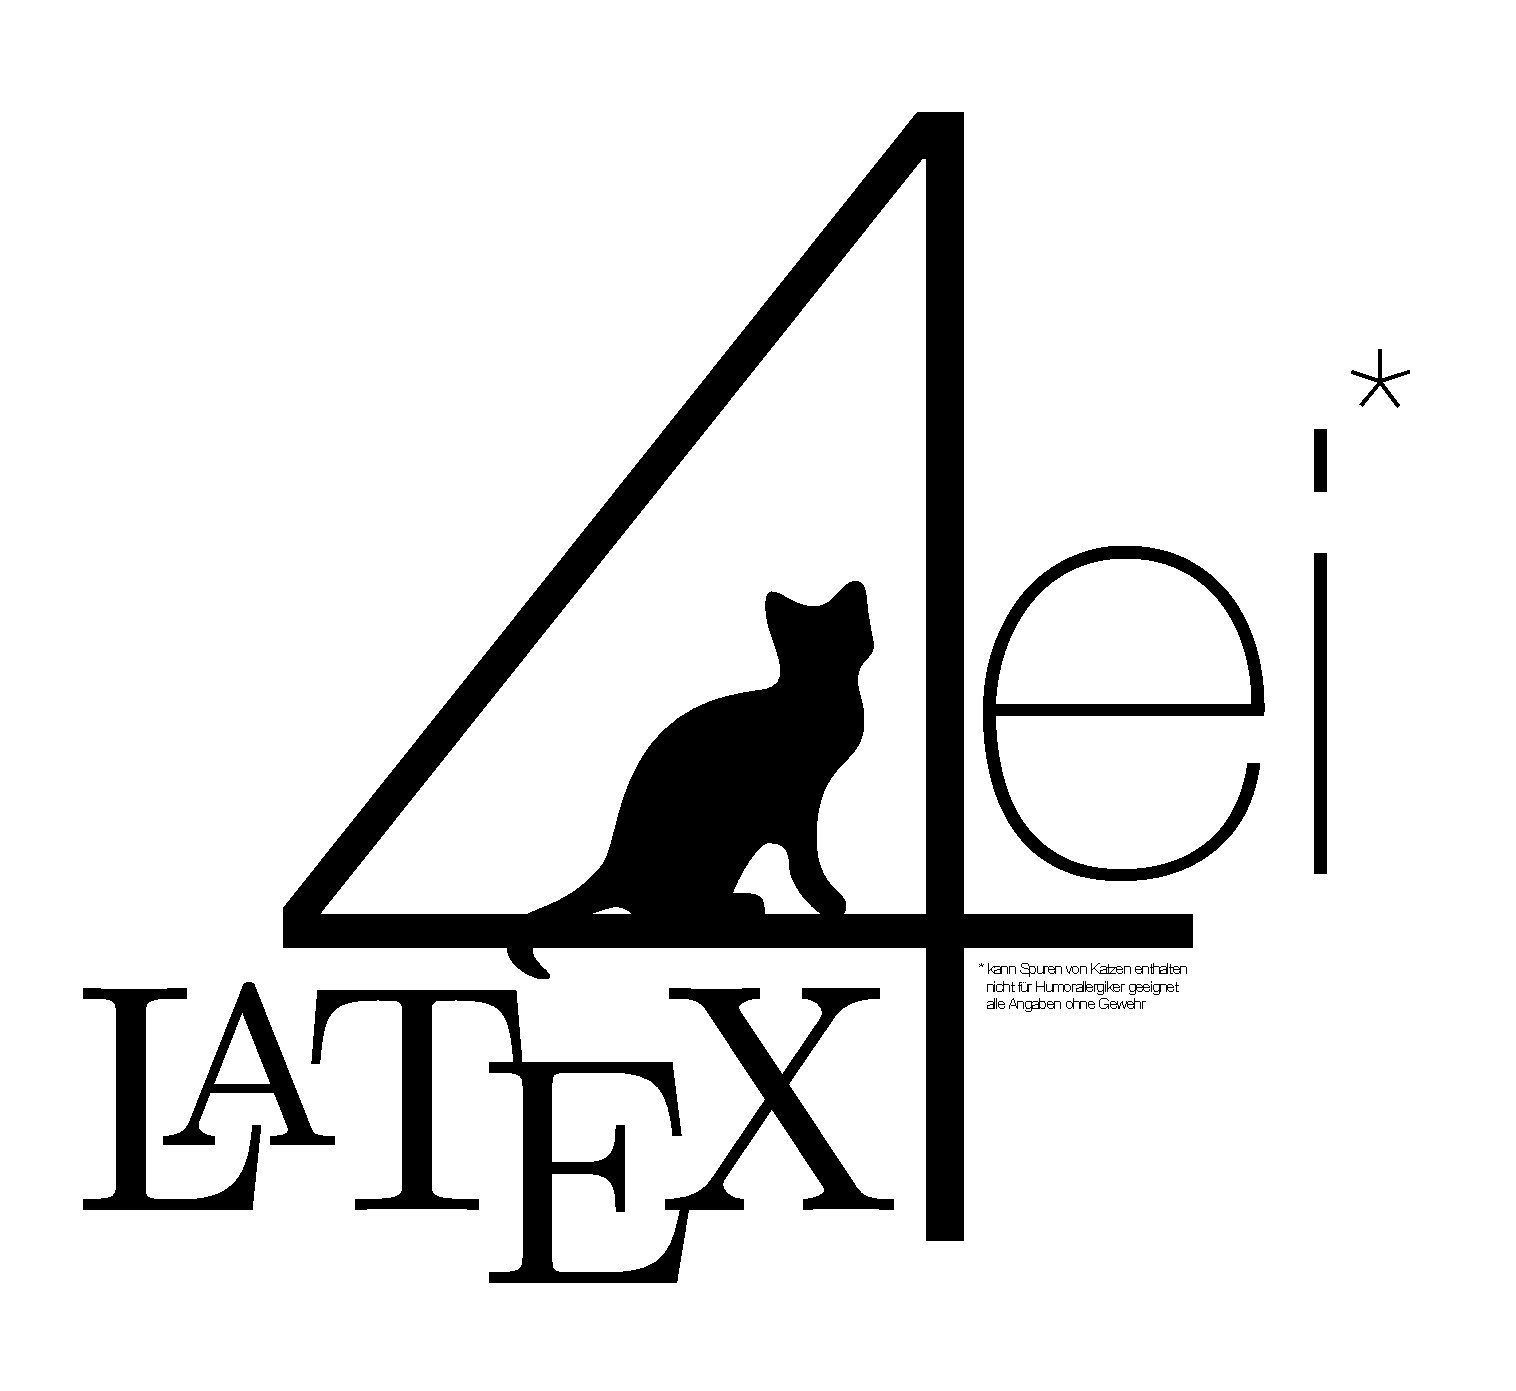
\includegraphics[height=1.4cm]{./img/Logo.pdf}		
	}
	\parbox{4cm}{
		\emph{\huge{Elektromagnetischer Feldterror}}
	}}
\vspace{-4mm} % Man muss optimieren wos nur geht ;)
% -------------------------------
% | 		EMF					|
% ~~~~~~~~~~~~~~~~~~~~~~~~~~~~~~~
%=======================================================================
\section{Nützliches Wissen $\rot E \equiv 0$}
Stromdichte $\vec j(\vec r) = \rho(\vec r) \vec v(\vec r)$\\
Elektrostatik heißt $\frac{\partial \vec D}{\partial t} = 0$, $\vec j = 0$ und Magnetostatik $\frac{\partial \vec B}{\partial t} = 0$ sonst spricht man von Elektrodynamik

\subsection{Konstanten}
\begin{tabular*}{\columnwidth}{@{\extracolsep\fill}ll@{}} \trule
	Lichtgeschwind. & $c = \frac{1}{\sqrt{\varepsilon_0 \mu_0}} = \SI{299 792 458}{\meter\per\second}$\\
	Elektr. Feldkonst. & $\varepsilon_0 = \SI{8.854 188e-12}{\farad\per\meter}$\\
	Magn. Feldkonst. & $\mu_0 = 4\pi \times \SI{e-7}{\henry\per\meter}$\\
\end{tabular*}

\subsection{Mathematik}
\hspace{-20pt}
\scalebox{0.77}
{
$\begin{array}{c|c|c|c|c|c|c|c|c|c|c|c}
x & 0 & \pi / 6 & \pi / 4 & \pi / 3 & \pi / 2 & \frac{2}{3}\pi& \frac{3}{4}\pi& \frac{5}{6}\pi& \pi  & \frac{3}{2}\pi & 2 \pi \\ \hline
\sin & 0 & \frac{1}{2} & \frac{1}{\sqrt{2}} & \frac{\sqrt 3}{2} & 1 & \frac{\sqrt 3}{2} & \frac{1}{\sqrt{2}} & \frac{1}{2} & 0 & -1 & 0 \\
\cos & 1 & \frac{\sqrt 3}{2} & \frac{1}{\sqrt 2} & \frac{1}{2} & 0 & -\frac{1}{2} & -\frac{1}{\sqrt 2}  & -\frac{\sqrt 3}{2}   & -1 & 0 & 1 \\
\tan & 0 & \frac{\sqrt{3}}{3}&1 &\sqrt{3} &  & -\sqrt{3}& -1& -\frac{1}{\sqrt{3}} & 0 &  & 0\\
\end{array}$
}
$z=a+b\mathbf{i}\ne0$\ in Polarkoordinaten:\\
$z=r (\cos(\varphi)+\mathbf{i}\sin(\varphi))=r\cdot e^{\mathbf{i} \varphi}$\\
$r=|z|=\sqrt{a^2+b^2}\quad\varphi=\arg(z)=\begin{cases}+\arccos \left( \frac{a}{r}\right),  & b\ge0   \\  -\arccos \left( \frac{a}{r}\right), & b<0\end{cases}$

\begin{description}\itemsep0pt
\item[Multiplikation:] $z_1\cdot z_2=r_1 \cdot r_2 ( \cos ( \varphi_1 + \varphi_2) + \mathbf{i} \sin (\varphi_1 + \varphi_2))$
\item[Division:] $\frac{z_1}{z_2}=\frac{r_1}{r_2} ( \cos ( \varphi_1 - \varphi_2) + \mathbf{i} \sin (\varphi_1 - \varphi_2))$
\item[n-te Potenz:] $z^n=r^n\cdot e^{n\varphi \mathbf{i}}= r^n (\cos (n \varphi) + \mathbf{i} \sin (n \varphi))$
\item[n-te Wurzel:] $\sqrt[n]{z}= z_k = \sqrt[n]{r} \left(\cos \left(\frac{\varphi + 2k\pi}{n}\right) + \mathbf{i} \sin \left(\frac{\varphi + 2k\pi}{n}\right)\right) \\ k =0,1, \ldots, n-1$
\item[Logarithmus:] $\ln(z)=\ln(r) + \mathbf{i}(\varphi + 2k\pi)$ \quad (Nicht eindeutig!)
\end{description}

\subsection{Maxwellsche Gleichungen (Naturgesetze)}
\setlength{\tabcolsep}{6pt}

\framebox[\columnwidth]{\vspace{0.3em}
	\begin{tabular*}{\columnwidth-4em}{@{\extracolsep\fill}ll@{}}
	Gaußsches Gesetz (inhom.) & Faradaysches ind. Gesetz\\
	\large $\div \vec D = \varrho $ & \large $\rot \vec E = - \frac{\partial \vec B}{\partial t}$ \\[1em]
	Quellfreiheit des magn. Feldes & Ampèrsches Gesetz (inhom.)\\
	\large $\div \vec B = 0$ & \large $\rot \vec H = \vec j + \frac{\partial \vec D}{\partial t}$\\[0.3em]
\end{tabular*} }\\
\\
Zusammen mit Materialgleichungen bildet
$(\vec E,\vec H)$ ein 6 komponentiges Elektromagnetisches Feld

\subsection{Materialgleichungen}

\subsection{Bauteilgleichungen}
\setlength{\tabcolsep}{6pt}
\begin{tabular*}{\columnwidth}{@{\extracolsep\fill}lll@{}} \trule
		\textbf{Resistiv} & \textbf{Kapazitiv} & \textbf{Induktiv}\\ \mrule
		\large $\mathrm d I = G \diff U$ & \large $\mathrm d Q = C \diff U$ & \large $\mathrm d \Phi_M = L \diff I$\\[0.3em] 
		\large $\vec j = \sigma \vec E$ & \large $\vec D = \varepsilon \vec E$ & \large $\vec B = \mu \vec H$\\ [0.3em] 
		\large $\mathrm d I = \vec j \diff A$ & \large $\mathrm d U = \vec E \diff \vec r$ & \large $\mathrm d \Phi_M = \vec B \diff A$\\[0.3em]  
		\large $\vec j = q n \vec v$ & \large $Q(V) \equiv \oiint\limits_{\partial V}\! \vec D \diff \vec A\;$ & \large $I(A) \equiv \oint\limits_{\partial A}\! \vec H \diff\vec r$\\ \noalign{\vspace{2pt}}\mrule
		Widerst. $R = \rho \frac{l}{A}$ & Kondens. $C=\frac{Q}{U} = \varepsilon \frac{A}{d}$ & Spule $L=\mu A \frac{N^2}{l}$\\
		 & $W_{el} = \frac{1}{2} C U^2$ & \\
		\pbox{3cm}{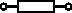
\includegraphics{./img/resistor.pdf}} & \pbox{3cm}{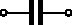
\includegraphics{./img/capacitor.pdf}} & \pbox{3cm}{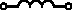
\includegraphics{./img/inductor.pdf}}\\ 
\end{tabular*}
\setlength{\tabcolsep}{4pt}

\everymath{\displaystyle} % Formeln ab hier groß Schreiben
\begin{tabular}{l|l|l}
	 & D-Feld & H-Feld \\ \hline
	Durchflutung & $\oiint_{\partial V} \vec D \cdot \mathrm d\vec a \equiv Q(V)$ & $\oint_{\partial A} \vec H \cdot \mathrm d\vec r=I(A)$ \\
	Vereinfacht & $4\pi r^2 D(r)=Q(V)$ & $2\pi r H(r)=I(A)$ \\
	Material & $\vec E = \frac{\vec D}{\varepsilon}$ & $\vec B = \mu \vec H$ \\
	Divergenz & $\mathrm{div}\ \vec D = \rho $ & $\mathrm{div}\ \vec B = 0 $ \\
	Rotation & $\mathrm{rot}\ \vec E + \frac{\partial \vec B}{\partial t} = 0 $ & $\mathrm{rot}\ \vec H = \vec j + \frac{\partial \vec D}{\partial t}$\\
\end{tabular}
\everymath{\textstyle} % Formeln ab hier normal Schreiben



\subsection{Formeln der Elektrostatik}
Coulombsches Gesetz: $\vec F = \frac{q}{4 \pi \varepsilon} \sum \limits_{i = 1}^N\frac{q_i (\vec r - \vec r_i )}{\abs{\vec r - \vec r_i}^3}$ \\
Elektrische Feldstärke: $\vec E = \frac{\vec F}{q} $ \quad $\rot E = 0$ \\
\textbf{Elektrostatische Felder sind konservativ} $\Leftrightarrow U = \Phi(P_1) - \Phi(P_2) = \int \limits_{P_1}^{P_2} \vec E d \vec r$ ist wegunabhängig \\
Potential: $\Phi (\vec r) = \frac{1}{4 \pi \varepsilon} \sum \limits_{i =1}^{N} \frac{q_i}{\abs{\vec r - \vec r_i}}$ \\
Poissongleichung: $\div(\varepsilon \grad(\Phi)) = - \varrho$ mit $\vec E = -\grad \Phi$ \\
Oberflächenladungsdichte: $\sigma = \vec D \cdot \vec N$ \\
Energie: $W_{12} = \int_C \vec F d \vec r = q \cdot U_{12}$ \\
Energiedichte: $w_{el} = \frac{1}{2} \vec E \vec D$ \\

\subsection{Formeln zu stationären Strömen}
$I = \frac{d Q}{d t} = \int \limits_A \vec j d \vec a$ mit Stromdichte $\vec j = qn\vec v = \abs{q}n\mu \vec E$ \\
Ohmsches Gesetz: $\vec j = \sigma\vec E$ \quad $U = R I$ mit $R = \frac{1 \cdot l}{\sigma\cdot A}$ \\
Verlustleistungs(dichte): $p_{\text{el}} = \vec j \vec E$ \quad $P = UI$ \\
Ladungsbilanzglg. (int, diff): $\int_{\partial V} \vec j d \vec a  = - \frac{d Q(V)}{dt}$ \quad $\div \vec j + \frac{\partial \varrho}{\partial t} = 0$

\subsection{Formeln der Magnetostatik}
Lorentzkraft(dichte): $\vec F_L = q \cdot (\vec v \times \vec B)$ \quad $\vec f_L = \vec j \times \vec B$\\
Elektromagnetische Kraft: $\vec F_{em} = q\cdot(\vec E + \vec v \times \vec B)$\\
Drehmoment einer Leiterschleife: $\vec M = I\vec A \times \vec B = \vec m \times \vec B$

\subsection{Formeln zur Induktion}
Magnetischer Fluss: $\Phi_{\text{mag}} = \int_A \vec B d \vec a$ \\
Bewegungsinduktion: $U_{\text{ind}} = - \frac{d \Phi_{\text{mag}}}{dt}$ \\
Ruheinduktion: $U_{\text{ind}} = - \int_{A(t)} \frac{\partial \vec B}{\partial t} d \vec a + \int_{\partial A(t)} (\vec v \times \vec B) d \vec r$

\subsection{Integralgleichungen}
nach Satz von Gauß: \\
$\int \limits_{\partial V} \vec D d \vec a = \int \limits_V \div \vec D d^3 r$ \\
$\int \limits_{\partial A} \vec H d \vec r = \int \limits_A \rot \vec H d \vec a$


\subsection{Durchflutungsgesetze:}
\boxed{\oiint\limits_{\partial V} \vec D \cdot \diff \vec a \equiv Q(V) } \qquad 
\boxed{\oint\limits_{\partial A} \vec H \cdot \diff \vec r = I(A) = \int\limits_{A} \vec j \diff \vec a}
\boxed { \div (\varepsilon \cdot \grad(\Phi)) = -\rho }




% .:: Das Elektrische Feld
%=======================================================================
\section{Das elektrische Feld}
\begin{enumerate}\itemsep-1pt
	\item Wird erzeugt von Ladung oder sich veränderndes Magnetfeld
	\item Innerhalb eines idealen Leiters ist das E-Feld Null(Influenz).
	\item Die Feldlinien stehen immer senkrecht auf eine Leiteroberfläche.
	\item Die Feldlinien laufen von positiven zu negativen Ladungen.
	\item Bei Kugelladungen sinkt das E-Feld radial mit $\frac{1}{r^2}$
	\item Bei unendlicher Linienladung sinkt das E-Feld radial mit $\frac{1}{r}$
	\item Bei unendlicher Flächenladung bleibt das E-Feld konstant.
	\item Feldlinien verlaufen lieber in hohem $\varepsilon_r$
\end{enumerate}

	% ------------------------------------------------------------------ 
	\subsection{Elektrische Energiedichte}
	Energie die in einem Bereich nötig ist, um alle Ladungen aus dem unendlichen an ihre Position zu bewegung.\\
	$W_{el} = \sum\limits_{k=2}^N \Delta W_{el}^{(k)} = \frac{1}{8\pi\varepsilon} \sum\limits_{\scriptscriptstyle \begin{matrix}\scriptscriptstyle i,k=1 \\[-0.3em] \scriptscriptstyle i \ne k\end{matrix}}^N \frac{q_i q_k}{|\vec r_i - \vec r_k|} = \iiint\limits_V \iiint\limits_V \frac{\rho(\vec r) \rho(\vec r')}{|\vec r - \vec r'|} \diff^3 r \diff^3 r'$\\
	\\
	\framebox[\columnwidth]{\pbox{\columnwidth}{
	Substitutionsregel:\\
	$q_i = \diff Q(\vec r_i) = \rho(\vec r_i) \diff V$\\
	$\sum\limits_{i=1}^N \{ \vec r_i ... \} q_i \ra \iiint\limits_V \{ \vec r_i ... \} \rho(\vec r) \diff V$} }\\
	\\
	$\delta W_{el} = \iiint\limits_V \Phi(\vec r) \delta\varrho(\vec r) \diff^3 r = \iiint\limits_V \vec E \cdot \delta \vec D \diff^3 r$\\
	
	
	\subsection{Energie}
	Die Gesamtenergie einer Ladungsverteilung mit $n$ Ladungen besteht aus $\frac{1}{2}(n^2 + n)$ summierten Termen.\\
	\begin{tabular*}{\columnwidth}{@{\extracolsep\fill}lll@{}} \trule
	& \large Elektrisch & \large Magnetisch\\ \mrule
				& $\delta w_{\ir el} = \vec E \cdot \delta \vec D$ & $\delta w_{\ir mag} = \vec H \cdot \delta \vec B$\\
		Energiedichte: & \boxed{ w_{\ir el} = \int\limits_0^{\vec D} \vec E' \diff \vec D' } & \boxed{ w_{\ir mag} = \int\limits_0^{\vec B} \vec H' \diff \vec B' }\\ \mrule
		$\begin{array}{@{}l} \text{Falls} \\ \varepsilon = \const \\ \mu = \const \end{array}$ & 
		$\begin{array}{@{}l} w_{\ir el} = \frac{1}{2} \vec E \vec D = \\ = \frac{\varepsilon}{2} \vec E^2 = \frac{1}{2\varepsilon} \vec D^2 \end{array}$ & 
		$\begin{array}{@{}l} w_{\ir mag} = \frac{1}{2} \vec H \vec B = \\ = \frac{\mu}{2} \vec H^2 = \frac{1}{2\mu} \vec B^2 \end{array}$\\ \mrule
		Energie: & $W_{\ir el} = \int\limits_V w_{\ir el} \diff V$ & $W_{\ir mag} = \int\limits_V w_{\ir mag} \diff V$\\ \brule
	\end{tabular*}\\ 
	\textbf{Leistung:} $P_{\ir em} = \int_V \Pi_{\ir em} \diff V = - \iint\limits_V \vec j(\vec r) \cdot \vec E(\vec r) \diff V$\\
	
	Energie eines Teilchens beim durchlaufen einer Spannung: $E = U \cdot Q$\\
	Energie des el. Feldes im Plattenkondensator: $E = \frac{1}{2} E D V = \frac{1}{2} U Q$\\
	
	\subsection{Elektromagnetisches Feld}
	\textbf{Poynting Vektor}: $\vec S := \vec E \times \vec H$\\
	Leistungsflussdichte: $\vec J_{\text{elmag}} = \vec E \times \vec H + \vec S_0$ ($\vec S_0 = 0$, falls voneinander unabhängige Quellen)\\
	Extensive Größe $X$ besitzt eine Volumendichte $x(\vec r,t)$, so dass für jedes Kontrollvolumen $V \subset \R^3$ gilt:
	$X(V) = \int_V x(\vec r,t) \diff V$\\ % ist die in V enthaltene Menge von $X$
	Extensive Größe ist eine Größe die man abzählen kann.\\
	\\
	Beispiele für extensive Größen:\\
	\begin{tabular*}{\columnwidth}{@{\extracolsep\fill}llll@{}} \mrule
	phys. Größe & $X$ & Volumendichte & $x$\\
	Ladung & $Q$ & Ladungsdichte & $\varrho_{el}$\\
	Masse & $m$ & Massendichte & $\varrho_m$\\
	Teilchenzahl & $N$ & Konzentration & $n$\\
	Energie & $W$ & Energiedichte & $w$\\
	\end{tabular*}	\\
	$X$ besitzt Stromdichte $\vec J_X(\vec r,t)$ mit $X = \vec J_X(\vec r,t) \diff \vec a$\\
	$X$ hat Produktionsrate $\Pi_X(\vec r,t)$ für Zeit und Volumen\\
	Bilanzgleichung: \boxed{ \frac{\diff X(V)}{\diff t} = -\int\limits_{ \partial V} \vec J_X \diff \vec a + \int\limits_V \Pi_X  \diff V}\\ 
	Differentielle Form: \boxed{\underset{\text{Akkummulationsrate}}{\frac{\partial x}{\partial t}} + \underset{\text{Zu-/Abfluss}}{\div \vec J_X} = \underset{\text{Generation}}{\Pi_X } }\\
	\\
	Halbleiter:\\
	Elektronen $\frac{\partial n}{\partial t} = -\div \vec J_n + G_n$\\
	Löcher $\frac{\partial p}{\partial t} = -\div \vec J_p + G_p$ mit $G_n = G_p$\\
	\\
	Energiebilanz des El.mag.-Feldes:\\
	\boxed{\frac{\partial w_{em}}{\partial t} + \div \vec J_{em} = \Pi_{em}}\\
	mit $w_{em} = w_{el} + e_{mag}$, $\vec J_{em} = \vec E \times \vec H + \vec S_0$, $\Pi_{em} = -\vec j \cdot \vec E$\\	


	\section{Potentialtheorie}
	Elektromagnetisches Vektorpotential $\vec A(\vec r, t)$: $\vec B(\vec r,t) = \rot \vec A(\vec r,t)$\\
	Elektromagnetisches Skalarpotential $\Phi$: $\vec E(\vec r,t) = - \nabla \Phi - \frac{\partial \vec A}{\partial t}(\vec r,t)$\\ 
	\\
	Umeichen: $\vec A' = \vec A - \nabla \chi$ \qquad $\Phi' = \Phi + \dot \chi$ \\
	
	Eichfunktion: Riemansche Räume haben an jedem Punkt ein anderes Längenmaß. Die Eichfunktion gibt an, welches Längenmaß an welchem Punkt verwendet werden muss.\\

	\subsection{Maxwell Gleichungen in Potentialdarstellung}
	\boxed{\div(\varepsilon \nabla\Phi) + \frac{\partial}{\partial t} \div(\varepsilon \vec A) = - \varrho}\\
	\boxed{\rot(\frac{1}{\mu} \rot A) + \varepsilon \frac{\partial^2 \vec A}{\partial t^2} + \varepsilon \nabla \frac{\partial \Phi}{\partial t} = \vec j }\\
	\\
	\textbf{Lorenzeichung:} $\div \vec A + \varepsilon \mu \frac{\partial \Phi}{\partial t} = 0$\\
	\\
	$\Rightarrow$ Wellengleichungen: \boxed{\left(\Delta - \varepsilon\mu \frac{\partial^2}{\partial t^2}\right) \vect{\Phi \\ \vec A} = - \vect{\frac{\varrho}{\varepsilon} \\ \mu \vec j }}\\
	\\
	\textbf{Coulombeichung:} $\div A = 0$\\
	$\Rightarrow$ Wellengleichungen: 
	\boxed{
	\begin{array}{lcl}
	\div\left( \varepsilon \nabla \Phi(\vec r,t) \right) = -\rho(\vec r, t) \text{ (Poisson)} \\ \\ 
	\Delta\vec A - \epsilon\mu\frac{\partial^2\vec A}{\partial t^2} = -\mu\left(\vec j - \epsilon\frac{\partial}{\partial t}(\nabla \Phi)\right)
	\end{array}
	}
	Elektromagn. Skalarpot. $\Phi(\vec r,t)$ folgt $\rho(\vec r, t)$ ohne Verzögerung!\\
	\\
	NF Anteil: $-\nabla \Phi$ \qquad HF Anteil: $\frac{\partial \vec j}{\partial t}$\\
	Transversale Stromdichte: $\vec j_t = \vec j - \varepsilon\frac{\partial \nabla \Phi}{\partial t}$\\
	
	%Fuck-Tor des Fickeschen Gesetzes:\\ 
	Gesetz bei dem Bert sabbert:\\
	$\vec H(\vec r) = \frac{I}{4 \pi } \int\limits_\gamma \frac{\diff \vec r \times (\vec r - \vec r')}{|\vec r - \vec r'|^3}$\\
	\\
	\sectionbox{
	\subsection{Feldverhalten an Materialgrenzen}
	\begin{center}
		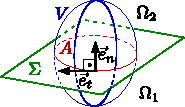
\includegraphics{./img/grenze2.pdf}
	\end{center} 
	Sprungbedingung für die Normalenableitung des Potentials:\\
	\begin{eqnarray*}
		\epsilon_1\frac{\partial \Phi}{\partial n}\big|_1 - \epsilon_2\frac{\partial \Phi}{\partial n}\big|_2 = \sigma_{\ir int} \text{ auf }\Sigma\\
	\end{eqnarray*}
	An Grenzflächen gibt es Flächenladung $\sigma:$ \\
	$Q = \lim\limits_{h \ra 0} \int_V \rho \diff V = \int_A \sigma \diff \vec a$\\
	\begin{eqnarray*}
	\vec D_2 \vec n - \vec D_1 \vec n = \sigma_{\ir int} \\
			\vec B_2 \vec n - \vec B_1 \vec n = 0 \\
			\vec E_1 \times \vec n - \vec E_2 \times \vec n = 0 \\
			\vec H_2 \times \vec n - \vec H_1 \times \vec n = \vec j
	\end{eqnarray*}
	Brechungsgesetz für elektrische Feldlinien (2 Isolatoren): \\
	\begin{eqnarray*}
		\frac{\tan \alpha_1}{\tan \alpha_2} = \frac{\varepsilon_1}{\varepsilon_2}
	\end{eqnarray*}
	}
	
	\subsection{Randwertprobleme der Potentialtheorie}
	Zu lösen ist die \textsc{Poisson}-Gleichung $\div(\varepsilon \nabla \Phi) = -\rho$ auf $\interior \Omega$:\\
	\begin{tabular*}{\columnwidth}{@{\extracolsep\fill}llll@{}}
	Nr. & RWP & Randbedingungen auf $\partial \Omega$ & Lösung\\
	1. & Dirichlet & $\Phi\big|_{\partial\Omega} = \Phi_D$ & eindeutig $\Phi \in \mathcal C^2$\\[0.5em]
	2. & Neumann & $\frac{\partial \Phi}{\partial \vec n}\Big|_{\partial\Omega} = F_N$ & eindeutig $(\Phi + C) \in \mathcal C^2$\\[0.5em]
	3. & Gemischt & $\left( \Phi + k \frac{\partial \Phi}{\partial \vec n}\right)\Big|_{\partial\Omega} = F_N$ & eindeutig $\Phi \in \mathcal C^2$\\
	\end{tabular*} 
	Mit Richtungsableitung $\frac{\partial \Phi}{\partial \vec n}\big|_{1/2} = \lim\limits_{\vec r - \vec r_0 \ra 0} \vec n(\vec r_0) \cdot \nabla\Phi(\vec r)$ \quad $\vec r \in \Omega_{1/2}$\\
	\\
	Lösungsansatz: $\Phi = \Phi^{(0)} + \varphi$\\
	$\Phi^{(0)}:$ erfüllt hom. DGL und inhom. RB\\
	$\varphi:$ erfüllt inhom. DGL und hom. RB\\
	\\
	In den meisten Elektrostatischen Problemen gilt $\rho = 0$, da sich die Ladung nur auf den Grenzflächen von Leitern befindet und nicht im Gebiet $\Omega$ in dem die Lösung von $\Phi$ gesucht wird.\\
	In der Praxis sind die meisten RWPs gemischt, wie Leiterkontakte oder Wärmeleitung\\ 
	
	Mehrelektroden-Kondensator Q-RWP:\\
	$\div(\varepsilon \nabla \Phi) = 0$ in $\interior \Omega$ und $\int_{\partial \Omega_l} \varepsilon \frac{\partial \Phi}{\partial \vec n} \diff \vec a = Q_l$ und  besitz bis auf eine additive Konstante eine eindeutige Lösung
	
	\subsubsection*{Spektralzerlegung}
	Lösungsverfahren:\\
	\begin{enumerate}
		\item Ansatz: $\Phi = \Phi^{(0)} + \varphi$\\
		Finde hinreichend glatte Funktion $\Phi^{(0)}$ welche inhomogene Randgleichungen erfüllt
		\item Finde Eigenfunktionen von $\varphi$: $f=-\div(\varepsilon \nabla \vec b_\nu) = \lambda_\nu \vec b_\nu$\\
			Es gilt $\lambda_\nu > 0$.
		\item Ansatz $\varphi(\vec r) = \sum_{\nu = 1}^\infty \alpha_\nu b_\nu(\vec r)$\\
		Bestimmung der Entwicklungskoeffizienten: $a_\nu = \frac{<b_\nu|f>}{\lambda_\nu} = \frac{1}{\lambda_\nu}\int_\Omega b_\nu * f dv$\\
		\item Spektraldarstellung: $G(\vec r, \vec r') = \sum_{\nu = 1}^\infty b_\nu (\vec r) \frac{1}{\lambda_\nu} b_\nu (\vec r')^*$\\
	\end{enumerate}
	
	
	
	\subsection{Greenfunktion $G(\vec r, \vec r')$}
	Def: Lösung des RWP mit hom. Randbed. und Störung $\rho(\vec r) = \delta(\vec r - \vec r')$ (Einheitspunktladung bei $\vec r'$)\\
	Poissongleichung $\Delta\varphi = -\frac{\rho}{\varepsilon_0}$ wird durch das Coulomb-Integral gelöst.
	Allg. Lösung: $\Phi(\vec r) = \int_\Omega G(\vec r, \vec r')\rho(\vec r') \diff^3 \vec r'$\\
	\\
	Beispiel Punktladung: $G_{\text{Vac}}(\vec r, \vec r') = \frac{1}{4 \pi \varepsilon} \frac{1}{\norm{\vec r - \vec r'}}$
	
	\subsubsection*{Spektralzerlegung mit Greenfunktion}
	Problem: \boxed{- \lpo \varphi = \tilde{f}}

	\begin{itemize}
		\item Sperationsansatz für die Eigenfunktionen: \\
		$b(\vec r) = b_1 (x_1) b_2(x_2) b_3(x_3)$
		\item $- \frac{\ddot b_1(x_1)}{b_1 (x_1)} - \frac{\ddot b_2(x_2)}{b_2 (x_2)}  - \frac{\ddot b_3(x_3)}{b_3 (x_3)} = \lambda$
		\item Aufteilen des Problems: \\
		$- \frac{\ddot b_1(x_1)}{b_1 (x_1)} = \lambda_1$ \\
		$- \frac{\ddot b_2(x_2)}{b_2 (x_2)} = \lambda_2$ \\
		$- \frac{\ddot b_3(x_3)}{b_3 (x_3)} = \lambda_3$
		\item Lösungsansatz für $b_1, b_2, b_3$: \\
		$b_j (x_j) = A_j \sin(k_j x_j) + B_j \cos (k_j x_j)$ mit $k_j = \sqrt{\lambda_j}$
		\item $\Ra B_j = 0$ und $k_j L_j = n_j \pi$
		\item Eigenfunktionen lauten: \\
		$b_j ( x_j ) = A_j \sin (n_j \frac{\pi}{L_j} x_j)$
		\item Normiere die Eigenfunktionen: \\
			$1 \overset{!}{=} \int \limits_0^{L_k} b_j (x_j)^2 \diff x_j$
	\end{itemize}
	
	Die Greenfunktion lautet nun: \\
	$G(\vec r, \vec r') = \sum \limits_{n_1, n_2 , n_3 \in \mathbb N} b_{n_1 n_2 n_3} (\vec r ) \frac{1}{\lambda_{n_1}\lambda_{n_2}\lambda_{n_3}} b_{n_1 n_2 n_3} (\vec r' )$
	%TODO S.52 Skript Lösungen der Laplace-Glg.
	\subsection*{Spiegelladungsmethode}
	Konstruktion eines Ersatzproblems durch Spiegelung der negierten Ladung an einer ebenen leitenden Randfläche\\
	%TODO S.63 Bild
	\begin{align*}
		G_{\text{Halb}}(\vec r, \vec r_0) = \frac{1}{4 \pi \varepsilon} \left( \frac{1}{\norm{\vec r - \vec r_0}} - \frac{1}{\norm{\vec r - \vec r_0^*}}\right)
	\end{align*}
	analog für Winkelräume. Eventuell müssen die gespiegelten Ladungen wieder gespiegelt werden (möglicherweise unendlich oft), bis sich alles ausgleicht.
	
	\subsection*{Multipolentwicklung}
	Coulomb-Integral: $\Phi(\vec r) = \int_{\R^3} G_{\ir vac}(\vec r, \vec r')\rho(\vec r') \diff^3 \vec r' = \frac{1}{4\pi\varepsilon_0}\int_{\R^3}  \frac{\rho(\vec r)}{\abs{\vec r - \vec r'}}\diff v'$\\
	Vereinfachung der Integraldarstellung durch Taylorentwicklung des Integralkerns $\frac{1}{\abs{\vec r - \vec r'}}$ unter der Annahme $\abs{\vec r'} < \abs{\vec r}$: 
	$\Phi(\vec r) = \frac{1}{4\pi\varepsilon_0}\frac{1}{r}Q + \frac{1}{4\pi\varepsilon_0}\frac{\vec r \cdot \vec p}{r^3} \mp \hdots$
	
	
	\subsection{Stationäre Ströme und RWP}
	Einflüsse: Drift, Diffusion, Hall-Effekt, Seebeck-Effekt\\
	Drift-Diffusionsmodell:\\
	\boxed{ \begin{array}{rll} \vec j = & \underset{\text{Driftstrom}}{\sum\limits_{\alpha = 1}^N |q_\alpha| n_\alpha \mu_\alpha \vec E} & - \underset{\text{Diffusionsstrom}}{\sum\limits_{\alpha = 1}^N q_\alpha D_\alpha \nabla n_\alpha} + \\[2em] + & \underset{\text{Halleffekt}}{\sum\limits_{\alpha = 1}^N \sigma_\alpha R_\alpha^H \vec \j_\alpha \times \vec B} & \underset{\text{Seebeck}}{-\sum\limits_{\alpha = 1}^N \sigma_\alpha P_\alpha \nabla T} \end{array}
	}\\
	$-\sum\limits_{\alpha = 1}^N \sigma_\alpha P_\alpha \nabla T$
	
	%$\sum\limits_{\alpha = 1}^N \sigma_\alpha R_\alpha^H \vec \j_\alpha \times \vec B
	
	
	\section{Kompaktmodelle}
	Modellierung als Netzwerk ohne Wellenausbreitung.\\
	Vorraussetzungen:\\
	\begin{enumerate}
		\item Räumlich begrenzte Funktionsblöcke:\\
			lokalisierte Schnittstellen (leitende Verbindungen, geführte elektromagnetische Felder)\\
		\item Quasistationär zeitveränderlich:\\
			Konzentriertheitshypothese: $\lambda >> d$.\\
			Knoten: ideal leitend, überall gleiches Potential.\\
			Zweige: flusserhaltend, gerichtete Spannung.\\
	\end{enumerate}
	
		\boxed{\lambda = \frac{c_0}{f}}
	
	
		\subsection{Kirchoffsche Gesetze}
		\boxed{ \sum U_i = U_{\ir ind} } \qquad \boxed{ \sum I_i = - \dot Q_K }\\
		
		\subsection{Kapazitive Speicherelemente}
		Mehrelektroden Kondensatoranordnung $\rightarrow$ Modellierung als Netzwerk von kapazitiven Zweipolen.\\
		Plattenkondensator: \\
		$\vec E = \frac{Q}{\varepsilon_0A}\vec\e$ \qquad $U = \int_0^d \vec E\diff\vec r = \frac{Q}{\varepsilon_0A}d$
		\begin{itemize}
			\item Kapazitätsmatrix:\\
				$C_{kl} = \int\limits_\Omega \nabla \Phi_k \varepsilon \nabla \Phi_l \diff^3 r = -\int\limits_{\partial\Omega_k} \epsilon \vec n \nabla \Phi_l d\vec a$ (k,l = 0, ..., N)\\
				$\ma C$ symmetrisch, positiv semi-definit, nicht invertierbar, Zeilen- und Spaltensumme null\\
			\item Reduzierte Kapazitätsmatrix:\\
				$\ma C_0: \ma C$ um 0. Zeile und 0. Spalte abgeschnitten\\
				$\vec U_0 = \mat{ V_1 - V_0 \\ \cdots \\ V_N - V_0 }$ \quad $\vec Q_0 = \ma C_0\vec U_0$ \quad $\ma C_0$ invertierbar\\
				
		\end{itemize}
		
		\subsection{Induktive Speicherelemente}
		$u_k(t) = -u_{\text{ind,k}}(t) + r_ki_k(t)$\\
		Transformatorgleichung: $u_k(t) = r_ki_k(t)+\sum_{l=1}^N L_{\ir kl} \frac{\diff i_l}{\diff t}$\\
		Kopplungsinduktivität: $M = k\sqrt{L_1L_2}$\\
		$\quad\Rightarrow U_1=L_1\dot{I}_1 + M\dot{I}_2\qquad U_2 = M\dot{I}_1+L_2\dot{I}_2$\\
		Neumannsche Formel: $L_{\text{kl}} = \frac{\mu}{4\pi}\int_{C_k}\int_{C_l} \frac{d\vec s' \cdot d\vec s}{\abs{\vec r - \vec r'(s)}} = \frac{\partial^2W_{\ir mag}}{\partial i_k\partial i_l}$ \\
		$L_{\text{kl}} : \begin{cases}\text{Selbstinduktionskoeffizient}, k=l\\\text{Gegeninduktionskoeffizient}, k \neq l\end{cases}$\\
		$\ma L$ symmetrisch, positiv definit
		
		
		
	\begin{tabular*}{\columnwidth}{@{\extracolsep\fill}ll@{}} \trule
		Kapazität & Induktivität\\
		$\vec Q = \ma C \vec U$ & $\vec \Phi_M = \ma L \vec i$\\
		$W_{\text{el}} = \frac{1}{2}\vec U_0\vec Q_0 = \frac{1}{2}\vec V^T\ma C\vec V$ & $W_{\ir mag} = \frac{1}{2} \vec I^\top \ma L \vec I$\\
		& $\boxed{ W_{\ir mag} = \frac{1}{2} \int\limits_{\R^3} \vec j \cdot \vec A \diff^3 r }	$
	\end{tabular*}\\



\section{Komplexe Wechselstromrechnung}
\textbf{Vorraussetzung:} lineares, eingeschwungenes System mit sinusförmiger Erregung $x(t) = A_m \cdot \cos(\omega t + \phi)$\\
Beim Kondensator eilt der Strom vor.\\
Bei der Induktivität kommt der Strom zu spät.\\
\sectionbox{
\subsection{Komplexe Zeigergrößen}
\emphbox{
	\begin{tabular}{ll}
	\textbf{Zeitfunktion} & $a(t) = A_m \cdot\cos(\omega t+\phi)$\\
	\textbf{Zeiger} & $A = \alpha + i\beta = A_m \cdot e^{i\phi}$\\
	&  $=A_m \cdot (\cos \phi+j\sin \phi)$\\
	\textbf{Maximum} & $A_m = |A| = \sqrt{\alpha^2+\beta^2} = \sqrt{AA^*}$\\
	\textbf{Phase} & $\phi = \begin{cases}
	\arctan\frac{\beta}{\alpha}&\alpha>0\\
	\arctan\frac{\beta}{\alpha}+\pi&\alpha<0
	\end{cases}$
	\end{tabular}
}

	% ---------------------------------------------------------
	Differentialoperator: $\frac{\diff}{\diff t} = j \omega$\qquad
	$\frac{d}{dt} e^{j(\omega t + \phi)} = j\omega\cdot e^{j(\omega t + \phi)}$\\
	\tablebox{
	\begin{tabular*}{\columnwidth}{l@{\extracolsep\fill}ccc} \ctrule
	 & \textbf{Widerstand} & \textbf{Kondensator} & \textbf{Spule}\\ \cmrule
	Impedanz $Z = \frac{U}{I} $ & $R$ & $\frac{1}{j \omega C}$ & $j \omega L$\\
	Admittanz $Y = \frac{I}{U} $ & $G = \frac{1}{R}$ & $j \omega C$ & $\frac{1}{j \omega L}$ \\[0.5em]
	$\underset{\varphi_u - \varphi_i}{\Delta \varphi =}$ & 0 & $-\frac{\pi}{2}$ & $\frac{\pi}{2}$ \\ 
				$\tan(\Delta\varphi) = \frac{\Im Z}{\Re Z}$\\
\cbrule
	\end{tabular*} 

	}
	\framebox[\columnwidth]{
		\begin{tabular}{l@{\hspace{4em}}l}
		$\underset{\text{Impedanz}}{\cx Z(j\omega)} = \underset{\text{Resistanz}}{R(j\omega)} + \underset{\text{Reaktanz}}{jX(j\omega)}$ & $\cx U = \cx Z \cdot \cx I$\\[1em]
		$\underset{\text{Admittanz}}{\cx Y(j\omega)} = \underset{\text{Konduktanz}}{G(j\omega)} + \underset{\text{Suszeptanz}}{jB(j\omega)}$ & $\cx I = \cx Y \cdot \cx U$\\
		\end{tabular}
	}
}
\sectionbox{
	\subsection{Komplexe Leistungsrechnung}
	$U_{\text{eff}} = \frac{1}{\sqrt{2}}U_m = \sqrt{\frac{1}{T}\int_0^T u(t)^2\diff t}$\qquad
	$I_{\text{eff}} = \frac{1}{\sqrt{2}}I_m$\\
	\textbf{Momentanleistung}: $p(t) = u(t)i(t)$\\
	\textbf{Energie einer Periode}: $E=\int_0^Tu(t)i(t)dt$\\
	\textbf{Leistungsmittelwert}: $P_w = \frac{1}{T} \int_0^T u(t)i(t)dt$\\
	\textbf{Komplexe Leistung}: $P = \frac{1}{2}UI^* = \frac{1}{2}U_m\cdot e^{j\varphi_u}\cdot I_m\cdot e^{-j\phi_i} = U_{\text{eff}}\cdot I_{\text{eff}}\cdot e^{j(\varphi_u-\varphi_i)}$\\
	\textbf{Scheinleistung}: $S = |P|$\\
	\textbf{Wirkleistung}: $P_w = \text{Re}\{P\} = \frac{1}{2}\hat U\hat I\cos \varphi$\\
	\textbf{Blindleistung}: $P_B = \text{Im}\{P\} = \frac{1}{2}\hat U\hat I\sin \varphi$
}

	\subsection{Grundlagen Wechselstromlehre}
	periodische, sinusförmige Strom- \& Spannungsverläufe:\\
	\begin{itemize}
		\item Transformierbarkeit(Energieübertragung) 
		\item Modulierbarkeit (Informations- und Nachrichtentechnik)
		\item Anpassung an Generatoren und Motoren
	\end{itemize}
	$\varphi(t) = \omega t + \varphi_0$ 



% .:: Elektromagnetische Wellen
%=======================================================================
\section{Elektromagnetische Wellen}
Transportieren Feldenergie mit Lichtgeschwindigkeit. $\varepsilon \mu c^2 = 1$\\ 
Unendliche Ausbreitung mit Lichtgeschwindigkeit ohne Medium.\\
Wechselwirkung mit der Materie.\\
Frequenzabhängigkeit von $\varepsilon(\omega),\mu(\omega),\sigma(\omega)$\\
Annahmen: $\rho = 0$ außer bei Antennen, keine thermischer Strom.\\

	\subsection{Beschreibung}
	\begin{tabular}{l@{\hspace{4em}}l}
		\ctrule
		Dämpfung & falls $\sigma > 0$\\
		äußere Quellen & $\vec j_0, \rho_0$\\
		\ctrule
		
	\end{tabular}
	
	6-Komponentiges, elektromagnetisches Wellenfeld:\\
	\boxed{ \mat{ \varepsilon \mu \frac{\partial^2}{\partial t^2} + \mu \sigma \frac{\partial}{\partial t} - \lpo } \vect{ \vec E \\ \vec H } = \vect{ - \nabla \left(\frac{\rho_0}{\varepsilon}\right) - \mu \dot{\vec j}_0 \\ \rot \vec j_0 } }\\
	Notwendig, aber nicht hinreichend für Maxwellsche Gleichungen. \\(Nebenbedingungen: $\varepsilon \div \vec E = \rho, \div \vec H = 0$)\\
	\\
	4-Komponentiges, elektromagnetisches Potential (falls $\sigma = 0$):\\
	\boxed{\left(\Delta - \varepsilon\mu \frac{\partial^2}{\partial t^2}\right) \vect{\Phi \\ \vec A} = - \vect{\frac{\varrho}{\varepsilon} \\ \mu \vec j }}
	
	Als Nebenbedingung muss nur die Eichbedingung erfüllt sein.\\
	
	homogene Wellengleichung: \boxed { \left(\frac{1}{c^2}\frac{\diff^2}{\diff t^2}-\Delta\right)\vec E = 0}
	
	\subsection{Eindimensionale Welle}
	Annahmen: $\sigma, \vec j_0,\rho_0 = 0 \Rightarrow \epsilon\mu \frac{\partial^2u}{\partial t^2}-\frac{\partial^2 u}{\partial x^2} = 0$\\
	Ausbreitungsgeschwindigkeit: $c = \frac{1}{\sqrt{\epsilon\mu}}$\\
	D'Alembertsche Lösung: $u(x,t) = f_1(ct-x)+f_2(ct+x)$\\
	\subsection{Dreidimensionale ebene Wellen}
	Annahhmen: $\sigma, \rho_0, \vec j_0 = 0$ \\
	Nebenbedingungen: $\div\vec E =\div \vec H = 0$ \quad $\rot \vec E = -\mu\frac{\partial\vec H}{\partial t}$ \quad $\rot \vec H = \frac{\partial\vec E}{\partial t}$\\
	\boxed{\vec k = k\vec n, \omega=kc} Dabei muss gelten: $\frac{\omega}{\abs{\vec k}} = c = \frac{1}{\sqrt{\epsilon\mu}}$\\
	$\vec E(t,\vec r) = \vec E_0(\omega t-\vec k\cdot\vec r)$ mit $\vec k\cdot\vec E_0(.) = 0$\\
	$\vec E_0(\vec r,t) =\frac{\vec k}{\epsilon \omega} \times \vec H_0(\vec r,t) = -Z\vec n \times \vec H_0(.)$\\
	$\vec H(t,\vec r) = \vec H_0(\omega t-\vec k\cdot\vec r)$ mit $\vec k\cdot\vec H_0(.) = 0$\\
	$\vec H_0(\vec r,t) =\frac{\vec k}{\mu \omega} \times \vec E_0(\vec r,t)= \frac{\vec n}{Z}\times \vec E_0(.)$\\
	Dispersionsrelation: $\omega(\vec k) = \frac{1}{\sqrt{\epsilon\mu}}\abs{\vec k}$\\
	Wellenwiderstand: $Z = \sqrt{\frac{\mu}{\epsilon}} = \frac{\abs{\vec E_0}}{\abs{\vec H_0}}$\\
	\subsubsection{Energie- und Leisungsbetrachtung}
	$w_{\ir el}(t,\vec r) = w_{\ir mag}(t,\vec r) = \frac{\epsilon}{2}\vec E_0(\omega t-\vec k\cdot\vec r)^2 = \frac{\mu}{2}\vec H_0(\omega t-\vec k\cdot\vec r)^2$\\
	Leistungsflussdichte: $\vec S = \frac{1}{Z}\vec E_0^2\cdot\vec n$\\
	Energiebilanz einer elektromagnetischen Welle: $\frac{\partial w_{\ir elmag}}{\partial t} + \div \vec S = 0.$\\
	\subsection{Harmonische ebene dreidimensionale Wellen}
	\subsubsection{Linear polarisierte Wellen}
	$\vec E(t,\vec r) = \vec E_0\cos(\omega t-\vec k\cdot\vec r + \varphi)$\\
	$\vec H(t,\vec r) = \vec H_0\cos(\omega t-\vec k\cdot\vec r + \varphi)$\\	
	\subsubsection{Elliptisch polarisierte Wellen}
	$\vec E(\vec r,t) = E_{01} \cos(\omega t -\vec k\cdot\vec r + \varphi_1) \vec e_1 + E_{02} \cos(\omega t - \vec k\cdot\vec r + \varphi_2) \vec e_2$\\
	%TODO Ab hier ists noch nicht gemacht	
	Harmonische, ebene EM Wellen ($\sigma = 0$)\\

	Ellipsengleichung:\\
	$\left(\frac{E_1}{E_{01}}\right)^2 + \left(\frac{E_2}{E_{02}}\right)^2 - 2\left(\frac{E_1}{E_{02}}\right)\left(\frac{E_1}{E_{02}}\right) \cos(\varphi_{02} - \varphi_{01}) = \sin^2(\varphi_{02} - \varphi_{01})$\\
	Linear: $\varphi_{02} - \varphi_{01} = n\pi$ \qquad $\frac{E_1}{E_{01}} = \pm \frac{E_2}{E_{02}}$\\
	Kreis: $\varphi_{02} - \varphi_{01} = (n+\frac{1}{2}) \pi \ \land \ E_{01} = E_{02}$ \qquad $\left(\frac{E_1}{E_{01}}\right)^2 + \left(\frac{E_2}{E_{02}}\right)^2$\\

	\subsubsection{Komplexe Darstellung}
	$\vec E(t,\vec r) = \Re{\underset{\hat E_0}{\underbrace{\left(E_{\ir 01}\e^{j\varphi_1}\vec\e_1 + E_{\ir 02}\e^{j\varphi_2}\vec\e_2\right)}\e^{j(\omega t-\vec k\cdot\vec r)}}}$\\
	\subsubsection{Darstellung beliebiger EM-Wellen durch harmonische ebene Wellen}
	Annahmen: $\varrho_0, \vec j_0 = 0, \sigma \geq 0$\\
	Materialgleichungen:
	\begin{itemize}
		\item $\vec D(\vec k) = \epsilon(\omega(\vec k))\vec E(\vec k)$
		\item $\vec B(\vec k) = \mu(\omega(\vec k))\vec H(\vec k)$
		\item $\vec j(\vec k) = \sigma(\omega(\vec k))\vec E(\vec k)$
	\end{itemize}
	komplexe Permittivität: $\tilde{\cx \varepsilon}(\omega) = \varepsilon(\omega) + \i \frac{\sigma(\omega)}{\omega}$\\
	komplexe Dispersionsrelation: $\tilde{k(\omega)}=\frac{1}{\tilde{\varepsilon}(\omega(\vec k))\mu(\omega(\vec k))}\vec k^2$\\
	komplexer Wellenwiderstand: $\tilde{Z}(\omega) = \sqrt{\frac{\mu(\omega)}{\tilde{\varepsilon}(\omega)}} = \frac{\tilde{k}(\omega)}{\omega\tilde{\varepsilon}(\omega)}$\\
	Fourierkoeffizienten der Feldgrößen:
	\begin{itemize}
		\item $\rot\vec E = -\frac{\partial\vec B}{\partial t} \overset{FT}{=} -j\vec k \times\hat{\vec E}(\vec k) = -j\omega\mu(\omega)\hat{\vec H}(\vec k)$, also $\vec k\times\hat{\vec E}(\vec k) = \omega(\vec k)\mu(\omega(\vec k))\hat{\vec H}(\vec k)$
		\item $\div\vec D = 0 \overset{FT}{=} -j\vec k\cdot\varepsilon(\omega)\hat{\vec E}(\vec k) = 0$, also $\vec k\cdot\hat{\vec E}(\vec k) = 0$
		\item $\rot\vec H = \vec j + \frac{\partial\vec D}{\partial t} \overset{FT}{=} \sigma(\omega)\hat{\vec E}(\vec k)+j\omega\varepsilon(\omega)\hat{\vec E}(\vec k) = j\omega\tilde{\varepsilon}(\omega)\hat{\vec E}(\vec k)$, also $-\vec k\times\hat{\vec H}(\vec k) = \omega(\vec k)\tilde{\varepsilon}(\omega(\vec k))\hat{\vec E}(\vec k)$
		\item $\div\vec B = 0 \overset{FT}{=} j\vec k\cdot\mu(\omega)\hat{\vec H}(\vec k) = 0$, also $\vec k\cdot\hat{\vec H}(\vec k) = 0$
	\end{itemize}
	inv. Dispersionsrelation: $\tilde{\cx k}(\omega) = \sqrt{\tilde{\varepsilon}(\omega)\mu(\omega)}$\\
	\subsubsection{Räumlich gedämpfte ebene EM-Welle in Leitern}
	$\tilde{\cx k}(\omega) = \underset{\text{Phasenmaß}}{\beta(\omega)} - \i \underset{\text{Dämpfungsmaß}}{\alpha(\omega)}$\\
	Näherung: $\sigma(\omega) \gg \omega\varepsilon(\omega)$\\
	$\alpha(\omega) = \beta(\omega) = \sqrt{\frac{\sigma(\omega)\mu\omega}{2}} = \frac{2\pi}{\lambda}$\\
	Eindringtiefe: $\Delta z(\omega) = \sqrt{\frac{2}{\sigma(\omega)\mu\omega}}$\\
	Abklingverhältnis: $\e^{-\lambda\alpha}$\\
	Skin-Effekt: Abschirmverhalten von leitenden Medien gegen das Eindringen von EM-Wellen
	\subsection{Einfall ebener elektromagnetischer Wellen auf ebene Materialgrenzschichten}
	Aufteilung der EM-Welle in reflektierenden und transmittierenden Anteil\\
	einfallend: $\vec H_h(\vec r) = \vec H_{\ir h0}\e^{-j\vec k_h\cdot\vec r}$, \qquad $\vec E_h = Z_1\vec H_h \times \e_{\ir kh}$\\
	reflektierend: $\vec H_r(\vec r) = \vec H_{\ir r0}\e^{-j\vec k_r\cdot\vec r}$, \qquad $\vec E_h = Z_1\vec H_h \times \e_{\ir kh}$
	transmittierend: $\vec H_D(\vec r) = \vec H_{\ir D0}\e^{-j\vec k_D\cdot\vec r}$, \qquad $\vec E_h = Z_2\vec H_h \times \e_{\ir kh}$
	%TODO Bild Skript S.163
	Reflexionswinkel gleich Einfallswinkel: $\alpha_h = \alpha_r$\\
	Brechungsgesetz (Snellius): $k_1\sin\alpha_h = k_2\sin\alpha_D$\\ \\
	\boxed{
		(\vec H_h + \vec H_r) \times \vec n = \vec H_D \times\vec n \qquad (\vec E_h + \vec E_r)\times n = \vec E_D \times \vec n
	}
	\textbf{E-Feld $\parallel$ Einfallsebene:} Einfallende Welle nennt sich TM-Welle\\
	%TODO Bild Skript S.165
	Reflexionskoeffizient: $r_{\parallel} = \frac{\hat E_r}{\hat E_h} = \frac{\hat H_r}{\hat H_h} = \frac{Z_2\cos\alpha_D - Z_1\cos\alpha_h}{Z_2\cos\alpha_D + Z_1\cos\alpha_h}$\\
	Transmissionskoeffizient: $t_{H\parallel} = \frac{\hat H_D}{\hat H_h} = \frac{2Z_1\cos\alpha_h}{Z_2\cos\alpha_D+Z_1\cos\alpha_h}$\\
	$t_{E\parallel} = \frac{\hat E_D}{\hat E_h} = \frac{Z_1}{Z_2}t_{H\parallel}$\\
	\textbf{E-Feld $\perp$ Einfallsebene:} Einfallende Welle nennt sich TE-Welle\\
	Reflexionskoeffizient: $r_\perp = \frac{\hat E_r}{\hat E_h} = \frac{\hat H_r}{\hat H_h} = \frac{Z_2\cos\alpha_h-Z_1\cos\alpha_D}{Z_2\cos\alpha_h+Z_1\cos\alpha_D}$\\
	Transmissionskoeffizient: $t_{E\perp} = \frac{\hat E_D}{\hat E_h} = \frac{2Z_2\cos\alpha_h}{Z_2\cos\alpha_h+Z_1\cos\alpha_D}$\\
	$t_{H\perp} = \frac{\hat H_D}{\hat H_h} = \frac{Z_1}{Z_2}t_{E\perp}$\\
	\subsection{Abstrahlung von EM-Wellen im freien Raum}
	Maxwellsche Gleichungen in zeitharmonischen Feldern:
	\begin{itemize}
		\item $\rot\vec E = -\j\omega\vec B = -\j\omega\mu_0\vec H$
		\item $\rot\vec H = \j\omega\vec D + \vec j_0 = \j\omega\varepsilon_0\vec E+\vec j_0$
		\item $\div\vec E = \frac{1}{\epsilon_0}\div\vec D = \frac{\varrho_0}{\varepsilon_0}$
		\item $\div\vec H = \frac{1}{\mu_0}\div\vec B = 0$
	\end{itemize}
	Helmholtz-Gleichung: $\Delta\vec A + \j\omega\varepsilon_0\mu_0\vec A = -\mu_0\vec j_0$\\
	Vereinfachung durch eingeprägte Dirac-Impuls Stromdichte der Form: $\vec j_0^D(\vec  r) = \hat I_0\Delta l\vec\e_z\delta(\vec r)$\\
	$\Rightarrow$ \textbf{Hertzscher-Dipol} mit Dipolmoment $I_0\Delta l$ mit $\vec A(\vec r) = \hat I_0\Delta l\mu_0\frac{\e^{-\j k_0r}}{4\pi r}\vec\e_z$\\
	%TODO Bild Skript S. 169
	
	\begin{description}
		\item[statisch:] Keine Veränderung über die Zeit $\frac{\partial}{\partial t} = 0$
		\item[stationär:] zeitliche Veränderung, aber keine Wellenausbreitung
		\item[Quasi-Stationär:] Zeitliche Veränderungen sind so langsam, dass sie als statisch angenommen werden $\frac{\partial}{\partial t} \approx 0$
		\item[Normalgebiet:] zusammenhängend, beschränkt, mit glattem lipschitstetigem Rand
		\item[Lipschitstetig:] irgendwas zwischen stetig und differenzierbar
	\end{description}
	$\mathcal L_2(\Omega) = \iset{f:\Omega \ra \C}{\int_\omega |f(\vec r)|^2 \diff^3 \vec r < \infty }$\\
	
	
	% Komplexe Wechselstromrechnung in der Prüfung!
	
	% Riemansche Zahlenkugel
	% Elektrische und Magnetische Felder können gesättigt werden!
	% Modell = kein Naturgesetz
	% Konforme Abbildung aus der Funktionentheorie zur Lösung der Poisson-Gleichung
	% r' ist r_0 also der Vektor vom Ursprung zur Ladung
	% Lipschitstetig ist irgendwas zwischen stetig und differenzierbar
	% IM vierdimensionen/quantenmachanik muss ein minus in den pythagoras
	% Ladung ist erste Komponente eines 4 dim Stromvektors
	%Minkovski Diagramm im Minkovski Raum
	%$\ma F^{\mu\nu} = \mat{0 & -\vec E_x & -\vec E_y & -\vec E_z \\ \vec E_x & 0 & - \vec B_z & \vec B_y \\ \vec E_y & \vec B_z & 0 & -\vec B_x \\ \vec E_z & -\vec B_y & \vec B_x & 0}$






%URI-QCU-PhiLI

% Zitate:
% Welche Vorraussetzungen müssen erfüllt sein, damit der Nossek funktioniert?
% Chemiker basteln Medikamente zusammen
% Die Ingenieure und die Maschinenbauer...

% Ende der Spalten
\end{multicols}

% Dokumentende
% ======================================================================
\end{document}

% ToDos:
% Leistungsdichte Vorzeichen
% Poynting-Vektor
% Energiebilanz elmag. Feld
% Leistungsfluss und Leistung
% Elektromagnetische Stromdichte
% Gleichung 1.46 & 1.48
% Gleichung 1.52 & 1.53 & 1.54 & 1.55 & 1.56 & 1.58
% Maxwellgleichungen in Potentialdarstellung
% 2. Poissongleichung
% EuM Schema
% Randwertproblem der Potentialtheorie
% Tabelle mit wichtigen Greenfunktionen

